\chapter{Consensus}\label{ch:consensus}
{
    \section{Introduction}
     {
      Previous Chapters discuss the scientific and technical aspects of CityScope, demonstrating how it can improve, expedite, and simplify complex urban processes. This last chapter concludes the \textit{New Urban Process} with the goal of using CityScope to establish consensus and agreement between diverse stakeholders. Too often, planning processes envision urban futures through data, simulation, and design iterations, but fail to include stakeholders and the general public as active voices in the decision-making \cite{Innes2016}. This is the byproduct of the length, complexity, and cost of traditional urban processes, as well as the fear of uncertainty and `anarchism' associated with the involvement of the masses \cite{banerjee2011companion}. In a traditional process, \textit{``the tasks are linear, and the players have separate and distinct responsibilities...(it) emphasizes getting the ``best'' and most objective information about an issue and using deductive logic to move from goals to choices.''} \cite{Innes2016} This status quo is deeply rooted in the assumption that the public is not necessarily aware or otherwise capable of comprehending the issues being addressed. With the immense flow of information, access to knowledge, and the ability to become a `citizen export' \cite{banerjee2011companion}, these notions are becoming obsolete in 21\textsuperscript{st} century urban-planning.


      \subsection{Citizen Participation}
      {
          As mentioned in Chapter \eqref{intro:challanges-processes}, even in democratic regimes, over-bureaucratization, privatization, and self-interests can create mistrust and discourage citizens from `real' involvement. In 1969, Arnstein proposed the `Ladder of Citizen Participation', a tool for evaluating and improving the engagement between citizens and stakeholders. Arnstein aimed to reflect on the range of participatory practices by inquiring - \textit{``What is citizen participation?...It is the redistribution of power that enables the have-not citizens, presently excluded...to be deliberately included in the future. It is the strategy by which the have-nots join in determining how information is shared, goals and policies are set...participation without redistribution of power is an empty and frustrating process.''} \cite{arnstein1969ladder}
      }

      \subsection{Resolving Impasses}
      {
          Arnstein's Ladder features eight `rungs' that describe three general forms of citizen power in decision-making: Nonparticipation (no power), Degrees of Tokenism (counterfeit power), and Citizen Power (actual power). Arenstein concluded that in many cases, participation ends within the bounds of tokenism, where citizens are either under the false perception of power-sharing, or are merely informed as passive observers. In higher levels of participation, \textit{``power is in fact redistributed through negotiation between citizens and powerholders. They agree to share planning and decision-making responsibilities through...mechanisms for resolving impasses.''} \cite{arnstein1969ladder}
          In this context, participation methods can address the need for \textit{`mechanisms for resolving impasses'}, which are set to reduce the friction between the public and decision-makers when providing equal access to information. The path leading form `passive' to `active' participation, can be achieved by the introduction of personal-learning and self-discovery \cite{bulmer_how_2001}. These promote the development of active learning and engagement systems, which bring participants to the center of the decision-making process.
      }

      \subsection{Collaborative Participation}
      {
          When moving from informing or consultation to active participation, the decision-making process gains the public's collective wisdom, while the public itself is empowered to make informed decisions \cite{innes2010planning}. This type of `Collaborative Participation' can gain from the usage of new tools, technologies, and data, as long as these are designed to facilitate the exchange and scrutiny of their own processes. As Inness concluded, \textit{``The potential for...adapting knowledge technologies to work for citizens is bounded only by our imaginations and possible only if technology itself is partially shaped by its users... we need to learn to take advantage of knowledge technologies for collaborative processes. To do so successfully will require that users shape and manipulate the technologies.''}\cite{innes2010planning} In that sense, collaborative platforms can only be viewed as a means to improve the quality of decision-making if the platforms themselves are open for review, evaluation, and even criticism.
      }
     }
    %%%%%%%%%%%%%%%%%%%%%%%%%%%%%%%%%%%%%%%%%%%%%%%%%%


    \section{Consensus Case Studies}
     {
      From its early prototypes (see Section \eqref{subsec:observatory_discussion}), CityScope development was centered around the engagement of diverse user groups. As explored in Chapter \eqref{ch:transformation}, the design of most CityScope instances followed this concept with user-friendly, accessible, and easily-extendable system. Nevertheless, these technical advantages cannot inherently promote a collaborative and consensus-driven process. Participation can only be viewed as a means to improve the quality of decision-making, if the process, tools, data, and models are themselves open and accessible \cite{Innes2016, innes2010planning}.
      \newline
      Early versions of CityScope evolved from a decades-long effort to create alternatives to traditional planning, design, GIS, and CAD tools \cite{ben-joseph2001, ishii2004bringing, negroponte1975soft, Sutherland1963}. For example, the Urban Observatory \eqref{sec:urbanobservatory}, CityScope Volpe \eqref{sec:cityscope_volpe}, and DeepScope \eqref{sec:deepscope} were all designed as reaction to the increased complexity, labor, and cost involved with traditional tools and their negative impact on urban processes as a whole.
      In 2014, CityScope was firstly suggested as an engagement platform for real-world public participation processes. \textbf{CityScope Boston BRT}, a community engagement and co-creation process for the planning on Bus Rapid Transit routes, brought together a range of UHCI technologies to be used in a public participation campaign. Here, CityScope was not only set as an alternative planning tool, but also as a medium supporting learning, debate, and evidence-based discourse by diverse and sometimes conflicting parties.
      \newline
      Many of the lessons learned in the BRT project, were put into extreme test in the \textbf{FindingPlaces} project. In 2015, the City of Hamburg faced an escalating crisis following a wave of refugees arriving from war zones in the Middle-East. CityScope FindingPlaces was created as part of a city-wide effort to engage the public on where-and-how should refugees be hosted in the future. FindingPlaces included a comprehensive public outreach, dozens of orchestrated community sessions, as well as structured documentation, feedback, and reporting mechanisms.
      \newline
      The rest of this Chapter discusses CityScope projects that demonstrated consensus-building, collaborative planning, co-creation, and learning with diverse stakeholders. It focuses on the role of CityScope within larger urban processes, and the impact it made both on the end-results, as well as the process itself.
     }

    %%%%%%%%%%%%%%%%%%%%%%%%%%%%%%%%%%%%%%%%%%%%%%%%%%
    \section{CityScope BRT}\label{sec:brt}
{
    \subsection{Introduction}
    {
        The development of improved transportation systems, particularly in undeserved communities, is a community engagement challenge \cite{jennings2004urban}. With many members of the public generally skeptical of government's ability to generate viable solutions, transport agencies and community organizations have been looking for ways to engage the general public on project proposals \cite{Innes2016}. One challenge is that existing tools for new public transportation proposals are mostly designed for professionals, hindering diverse stakeholders to understand, evaluate, and provide feedback on the benefits and tradeoffs of the plan.
        \newline
        With support from the City of Boston and the Barr Foundation, \textbf{CityScope BRT} proposed several interactive urban-planning tools to explore the potential for implementing new Bus Rapid Transit (BRT) in different parts of the City of Boston \cite{stewart2018tangible, Newinter52:online}. Three tools were devised for the exploration of multiple urban scales: the regional, neighborhood, and street level. Partnering with Nuestra Communidad \cite{nuestracdc:online}, a local community organization, the tools were deployed in a public participation process, which was designed to test the potential benefits of CityScope as an alternative medium for community planning, co-creation, and learning \footnote{This project was conceived jointly between the MIT Department of Urban Studies and Planning, the MIT Media Lab, Nuestra Communidad board members, and the Barr foundation. The project was hosted in a space provided by the Roxbury Innovation Center.}.


        \begin{figure}[!htb]
            \begin{center}
                \includegraphics[width=1\textwidth]{chapters/consensus/BRT/figures/brt2.jpeg}
            \end{center}
            \caption{Boston BRT timeline. The community engagement process started months before the actual BRT workshops took place, with activities, co-creation, and constant deliberation with stakeholders and community members. (right) A member of the public operates the BRT Street Scale platform.}
            \label{fig:brt_exit_timeline}
        \end{figure}


        \subsubsection{Research Objectives}
        {
            This project seeks to determine how facilitator-led, collaborative use of new tools might encourage public engagement. Specifically, The research investigates mechanisms to promote social learning, co-creation, and consensus among stakeholders, using collaborative tools in public workshop settings. Potential engagement mechanisms include: (i) Specific features, such as options for localization and interaction based on personal experience; (ii) Tool-supported group interactions, such as discussion and comparison of impacts between user-relevant locations; and (iii) General promotion of understandability, personalization, discussion, teamwork, credibility, and imagination. In testing these mechanisms, participant-reported scores for learning and open dialog are determined from pre-and-post session surveys.
        }


        \begin{figure}[!htb]
            \begin{center}
                \includegraphics[width=1\textwidth]{chapters/consensus/BRT/figures/brt7.jpeg}
            \end{center}
            \caption{Features of BRT systems \cite{Aboutthe77:online}. At full implementation, a BRT system will feature pre-payment systems, enhanced stations and stops, dedicated lanes, all-door boarding, digital payments, and other features making the BRT experience closer to the performance and convenience of heavy transit solutions.}
            \label{fig:brt_what_is_BRT}
        \end{figure}


        \subsubsection{Bus Rapid Transit}

        {
            Improved bus service can support urban expansion at relatively low cost compared to other mass-transit solutions \cite{williams2015better}. Examples of high quality, bus-based, surface-level public transit exist worldwide, from Mexico City to Malmö (Sweden), and from Cleveland to Cape Town \cite{wirasinghe2013bus}. As Figure \eqref{fig:brt_what_is_BRT} show, these Bus Rapid Transit systems (BRT) tend to include dedicated bus-lanes and pre-payment systems at quality stations. The BRT Standard defines several dozen individual characteristics that the Technical Committee has deemed essential to the definition of BRT. Each is assigned a point value if present; When totaled, the highest scored projects are categorized as `Gold Standard,' followed by `Silver Standard,' and lastly `Bronze Standard.' \cite{Aboutthe77:online}.
            Despite its promise, some aspects of BRT are still controversial: Operating on streets long-dominated by cars can pose difficult tradeoffs in terms of street-scape allocation. BRT might require the removal of existing car lanes or parking spots, change to travel time for car riders, and infrastructural changes to the streetscape \cite{wirasinghe2013bus}.
            \newline
            In 2015, the Greater Boston Bus Rapid Transit Study Group published a report titled \textit{``Better Rapid Transit for Greater Boston: The Potential for Gold Standard Bus Rapid Transit across the Metropolitan Area''} \cite{williams2015better} This document offers a city-wide technical analysis of BRT, and recommends five specific corridors for further evaluation and future implementation. Following the report, The Barr Foundation requested to explore how the use of interactive tools could facilitate the engagement with the community on the wider implications of developing these routes.
        }

        \subsubsection{Site and Context}
        {
            The Roxbury Innovation Center (RIC), Located in the new Bolling Municipal Building in Roxbury (Boston, MA), was selected as the venue location for the community engagement process. RIC sits adjacent to a major bus transportation hub, which is planned to serve several BRT future routes.
            The Roxbury neighborhood has been underserved by transportation and socio-economic mobility for the past several decades \cite{jennings2004urban}. Though Roxbury communities are served by several MBTA bus routes, these operate in mixed traffic and therefore are considerably slower than existing rapid transit lines. Of the fifteen bus routes that are designated by the MBTA as `Key Bus Routes', six provide service in Roxbury, Dorchester, or Mattapan. Five of the MBTA's seven highest ridership bus routes operate primarily within these neighborhoods \cite{MapsMBTA95:online}. These routes tend to suffer from poor reliability, slow travel speeds, overcrowding, and a lack of customer amenities \cite{SurveyBo15:online}. Of the five potential corridors proposed in the BRT Study Group report, three converge at the Dudley Square station, making Roxbury an ideal community for stakeholders engagement in the evaluation of BRT potential \cite{williams2015better}.
        }
    }

    \begin{figure}[!htb]
        \begin{center}
            \includegraphics[width=1\textwidth]{chapters/consensus/BRT/figures/brt0.jpeg}
        \end{center}
        \caption{CityScope BRT. Three CityScope instances were proposed to allow simultaneous discussions in multiple scales and different impact levels of the BRT system. The three platforms also presented a gradual move from an intuitive street-scale tool to a more detailed and complex regional platform.}
        \label{fig:brt_platforms}
    \end{figure}

    \subsection{CityScope Tools}
    {
        A set of tools was developed in an effort to test collaboration and co-creation using digital platforms in the context of BRT planning. These include CoAXs \cite{stewart2016coaxs}, a web-based interactive platform for collaborative transit planning\footnote{CoAXs was built upon the open-source urban analytics tool Conveyal \cite{Conveyal33:online}. For a detailed description of CoAXs, see \cite{stewart2016coaxs}}. The second set of tools were two CityScope platforms, designed for the neighborhood and street-level scales. These offered an iterative way to examine alternatives for bus corridor designs, station types, street layouts, as well as travel times and environmental impacts. CityScope visualized traffic based on the outputs of different analysis tools such as SUMO, an open source traffic modeling software \cite{krajzewicz2012recent}. The following section details the tools and their functionality.

        \begin{figure}[!htb]
            \begin{center}
                \includegraphics[width=1\textwidth]{chapters/consensus/BRT/figures/brt4.jpeg}
            \end{center}
            \caption{CoAXs regional scale UI. These screen-captures show the control panel and interaction with the CoAXs touch screen interface, with results from the Conveyal accessibility service, including assessed travel time, access to different amenities and functions, as well as estimated cost.}
            \label{fig:brt_street_CoAXs}
        \end{figure}

        \subsubsection{CoAXs: Regional Scale}
        {
            CoAXs (short for `Co-Creative Accessibility-Based Stakeholder Engagement') is a web-based mapping and visualization tool designed to evaluate and communicate benefits of transit projects in collaborative planning. CoAXs seeks to link maps and accessibility indices with various common travel patterns. For example, viewers can point to a specific location in the city (via interactive touch interface) and learn their access to job locations given proposed public transportation. They can then control various model assumptions (such as bus frequency) to see how different transit systems and route networks affect their commute as well as overall job accessibility.
            \newline
            CoAXs has two modules: (i) the accessibility analyst, synthesize data about transit service, pedestrian and cycling networks, land-use, and socio-economics, to provide interactive maps of both individual access to opportunities and regional accessibility; (ii) a sketch-planning corridor editor that allows users to modify the service parameters of bus corridors and create different corridors` scenarios.
            CoAX is built using Conveyal's Transport Analyst and Open Trip Planner \cite{Conveyal33:online}.
        }


        \begin{figure}[!htb]
            \begin{center}
                \includegraphics[width=.8\textwidth]{chapters/consensus/BRT/figures/brt11.jpeg}
            \end{center}
            \caption{Neighborhood Scale. This TUI responded to users' changing the BRT tiers with highlighted routes, travel times, cost, and environmental impacts. Between the three platforms, the Neighborhood scale was the least useful, as the tangible interface did not contribute to the understanding of the BRT system, and the coarseness of the model was found to be confusing.}
            \label{fig:brt_neighborhood_scale}
        \end{figure}


        \subsubsection{CityScope: Neighborhood and Street Scales}
        {
            Two CityScope instances were designed for the analysis of BRT systems, neighborhood and street Scales. These complement the CoAXs modules, and allow users to explore the potential impacts of different BRT configurations and route networks of neighborhoods and streets.


            \begin{figure}[!htb]
                \begin{center}
                    \includegraphics[width=1\textwidth]{chapters/consensus/BRT/figures/brt6.jpeg}
                \end{center}
                \caption{BRT `Street-Scale'. As users interact with the TUI (right), both the projection and AR device (left) update information about the impacts of the different BRT tiers.}
                \label{fig:brt_street}
            \end{figure}

            \textbf{Neighborhood:} The Neighborhood scale is designed to explore the accessibility created using new BRT routes in the vicinity of the Roxbury area. This scale provides users with a design-decisions interface around selection of street corridors, placement and sizing of stations, and improving overall utilization of transit systems. A 3D neighborhood scale model was fitted with several placements for inserting LEGO tiles, which refer to BRT stations in key locations across the city. Each of the bricks would represent one of three BRT station standards (Gold, Silver, or Bronze. See \cite{Aboutthe77:online}). When users place a station onto the designated spot, the corresponding BRT route and its stations are displayed. In addition, recorded BRT trips simulation is playing, showing a fast-paced visualization of the proposed routes for this BRT class. The selected type of the BRT class also impacts several precalculated metrics, such as the number of passengers served, the number of trips per hour, as well as environmental impacts. These are displayed on auxiliary monitors.

            \begin{figure}[!htb]
                \begin{center}
                    \includegraphics[width=1\textwidth]{chapters/consensus/BRT/figures/brt3.jpeg}
                \end{center}
                \caption{Street-Scale TUI screen-captures. (top) Washington st. in its current state, including the performance of the MBTA Silver Line, available parking, and bike access. (bottom) Washington st. fitted with a `BRT Gold Standard', including improved transit times and accuracy, enhanced bike access, and tradeoffs to private vehicles.}
                \label{fig:brt_street_viz}
            \end{figure}

            \textbf{Street:} The second instance focuses on the street-level impacts of a BRT corridor. This street section was modelled after a segment of Washington st., which included an existing MBTA Silver Line bus route. Here, users are promoted to engage in design-decisions such as placement and sizing of various stations, streetscape design, bike-able access to BRT stations, and increasing access for seniors, disabled, and youth. Users can switch out different pieces representing various types of bus stops (from traditional ones to high-tech stations where riders pay before they board) and observe the simulated change in traffic flow on the LEGO platform. Data about the bus station's efficiency is also projected on nearby screens, as well as on the CityScopeAR platform \cite{nsl19}.
        }
    }

    \subsection{Workshops}
    {
        The development of the different tools took place during the first half of 2015. As part of the engagement process, Boston high school students participating in the MLK Scholars program, constructed the neighborhood scale LEGO model of Roxbury. Between June and October, several review sessions and workshops were held at the MIT Media Lab, hosting stakeholders, members of the community, and students participants. In September, the three tools were deployed to the venue site, and facilitators training session took place at MIT and on the venue premise. During October, six workshops, involving 53 participation, took place in the venue. Alongside the workshops, the venue was open for members of the community to explore the CityScope tools and learn about the proposed BRT system. The following section details the workshops, agenda, and feedback collection.

        \subsubsection{Facilitators}
        {
            Typically problematic of government-run community meetings is the perception that control of the technology, and therefore the analyses, is in the hands of technical experts \cite{innes2010planning, arnstein1969ladder}. By combining interactive tools with community facilitators, participants' perception of tools credibility and empowerment to play a more active role in planning their own community was tested.
            \newline
            A key element of the workshops was the partnership with Nuestra Communidad \cite{nuestracdc:online} who provided six members as facilitators for the workshops. Rather than have researchers engaging the public, community leaders facilitated the workshops sessions and operated the tools by themselves. Two training sessions were held with the facilitators prior to the workshops; An unintended benefit of these training sessions was the valuable feedback on the tools' usability, readability, and accessibility.
        }

        \begin{figure}[!htb]
            \begin{center}
                \includegraphics[width=1\textwidth]{chapters/consensus/BRT/figures/brt8.jpeg}
            \end{center}
            \caption{The many faces of public participation. A key aspect of this project was the engagement of stakeholders and the general public in every phase, from initiation and design to execution and evaluation.}
            \label{fig:brt_public_grid}
        \end{figure}

        \subsubsection{Workshops Agenda}
        {
            All six workshops followed a similar structure:
            \newline
            \textbf{Registration:} As participants entered, they were asked to register, which included reading and signing a consent to participate in the research and filling out a pre-workshop survey. Participants were also asked to use a tablet to map their points of interest (e.g., home, work, school, recreation, and healthcare locations) saved for later use in the workshop with the CoAXs tool. Participants were then asked to freely wander and familiarize themselves with the facilitators, space, and tools.
            \newline
            \textbf{Orientation:} Participants were first given an opportunity to introduce themselves to each other. One of the researchers then presented an overview to transportation issues facing Boston and the Roxbury neighborhood, explanation of the purpose of the project and project team, and introduction to key elements of Bus Rapid Transit systems.
            \newline
            \textbf{Exploration using BRT Tools:} Participants were divided into three groups. Each group was told to start at a particular station and then rotate to another station after 20 minutes. A member of the research team and a community facilitator from Nuestra was at each station helping to facilitate the conversation.
            \newline
            \textbf{Debrief discussion:} At the end of each workshop, all participants gathered for a facilitated debrief of the experience. One of the researchers facilitated each of these sessions with open-ended questions. Attempts were made to engage each of the participants during this closing session.
            \newline
            \textbf{Post-workshop survey:} Before leaving, participants were asked to fill out a post-workshop survey, including open-ended feedback as well as five-point Likert-type scales to report various takeouts and concerns. The survey was designed to be anonymous and was used to generate the report of the workshop.
        }

        \subsubsection{Data collection}
        {
            There were three primary methods to collect data during the workshops: (i) the written pre- and post-workshop surveys, (ii) verbal feedback provided during the debrief session, and (iii) observations and video/audio recordings. The pre-workshop survey collected some basic demographics, and a senses of previous familiarity with visual representation of information, public meetings, and Bus Rapid Transit. The post-workshop survey consisted of two sections: one asked questions about the overall experience of the workshop, and the second asked a series of identical questions about each of the three stations.
        }
    }

    \subsection{Results}
    {
        A mixed-method analysis suggests that the constructs of plausibility (credibility and fostering imagination) and alignment (discussion and teamwork) are correlated with specific interactions \cite{Alrashed2015}. These findings, while not robustly generalizable, suggest that stakeholder engagement built around collaborative tools, has the potential to improve processes of decision making in the context of city-planning. This section discusses the results of the workshops, including the analysis of the data collected from surveys and observations.


        \begin{figure}[!htb]
            \begin{center}
                \includegraphics[width=1\textwidth]{chapters/consensus/BRT/figures/brt9.jpeg}
            \end{center}
            \caption{Participants demographic breakdown.}
            \label{fig:brt_demographics}
        \end{figure}

        \subsubsection{Participant Characteristics}
        {
            Six workshops were held with 53 total participants from a range of advocacy, policy, neighborhood, and professional organizations. Of these participants, 13 were classified as transportation, policy, or planning experts, and 15 reported attending no public planning meetings within the preceding year. Pre-workshop surveys collected basic demographics: Participants ranged in age from under 21 to over 75, though the bulk of participants were between 21 and 54. There was a diverse range of professions reported overall: About 20\% identifying as an engineer, architect, planner, transportation professional, or consultant, and 10\% identifying as a student. Almost three quarters answered yes to the question, \textit{``Are you familiar with the concept of Bus Rapid Transit (BRT)?''}
        }

        \subsubsection{Overall Responses}
        {
            Overall responses about the workshops were positive. The two questions that generated the most neutral or negative responses had to do with the role of the individual: \textit{``I helped others learn''} and \textit{``I feel that I can play an active role in the community where I live.''}
            The usage of tools was meant to assess multiple types of learning. ``Single-loop'' learning takes place when the focus is on improved techniques of efficiency (technical rationality), and goals, values, and strategies are taken for granted \cite{greenwood1998role}. The following question is taken to measure factual learning, also called `reported learning', and is associated with instrumental and strategic rationality. Nearly three quarters of participants reported positively to this question: \textit{``I learned a great deal in the workshop.''}
            \newline
            ``Double-loop'' learning is associated with communicative and value rationality. Four survey questions were used together to assess this type of learning, associated with a set of ``governing variables'': valid information, free and informed choice, internal commitment to choice, and evidence seeking behavior\footnote{Learning questions were asked for the overall workshop, since it might have been difficult for participants to isolate what they learned using an specific tool versus the workshop introduction, etc.}. The following responses signal a measure of communicative learning:

            \begin{itemize}
                \item \textit{I was able to get answers to the questions I asked} [Evidence seeking]
                \item \textit{Workshop participants discussed issues in an open way} [Valid information]
                \item \textit{Participants were open to differences in opinion} [Free and informed choice]
                \item \textit{I would support recommendations created by the participants of the workshop} [Internal commitment to choice]
            \end{itemize}

            Where valid responses were present from all questions, these were summed to create a double loop index, with possible values ranging between 4 to 20. Taken together, the answers to these questions suggest a positive response to higher-level learning. The traditional measure of the internal consistency of a scale used widely in social research, is the Cronbach alpha coefficient, which is a direct function of the number of items and their inter-correlation. The coefficient takes values between 0 and 1, and higher values correspond with higher internal consistency. An accepted rule of thumb for internal consistency, is a value of at least 0.70. The alpha value for the four statements listed above was 0.78 \cite{brown2002cronbach}.
        }

        \begin{figure}[!htb]
            \begin{center}
                \includegraphics[width=1\textwidth]{chapters/consensus/BRT/figures/brt10.jpeg}
            \end{center}
            \caption{Learning outcomes. Overall, the vast majority of participants reported increase in `double loop' learning, awareness, and understanding of the BRT system.}
            \label{fig:brt_learning_outcomes}
        \end{figure}

        \subsubsection{Learning and Predispositions}

        {
            Participants bring with them different predispositions, such as current knowledge and attitudes. A hypothesis for this project is that the CityScope tools will encourage a different amount of learning across these differences. Responses to reported learning were segmented by past planning experiences, including along (i) expert/non-expert and (ii) skeptic/non-skeptic lines. Neither of these distinctions was asked explicitly on the entry survey; Transportation, policy, and planning experts were identified based on participants' open-ended description of their professions. Thirteen participants (about one third) were classified as ``experts'', interpreted as coming with existing transportation planning or engineering professional experience; 32 as ``non-experts,'' interpreted as coming from another discipline or life experience.
            \newline
            In general, non-experts reported more single-loop learning. For skepticism, participants were asked how many planning meetings they had attended in the preceding year, and the number of these meetings at which they learned something about this project. The difference between the former and the latter was deemed an imputed measure of skepticism about learning in planning meetings, and participants with a difference greater than zero were classified as skeptics (a binary variable). Nearly 20\% were classified as ``skeptics''; Consistent to expectations, non-skeptics reported more single-loop learning, and few reported a ``1'' (did not learn anything in the workshop).
        }


        \begin{figure}[!htb]
            \begin{center}
                \includegraphics[width=1\textwidth]{chapters/consensus/BRT/figures/brt1.jpeg}
            \end{center}
            \caption{Aggregated results from exit surveys. Participants reflected on their learning outcomes and attitudes towards the BRT system in comparison to their initial perception. They rate each of the CityScope tools as well as cumulatively evaluate their learning from the overall experience.}
            \label{fig:brt_exit_survey}
        \end{figure}


        \subsubsection{Comparative Evaluation of Tools}
        {
            The post-workshop survey included a series of questions about each of the tools (regional, neighborhood, and street scale). Overall, the participants reported a positive experience with all tools. These are some anecdotal findings from the surveys:

            \begin{itemize}
                \item The street-scale appeared to be the easiest and most accessible to understand;
                \item The regional-scale scored the highest overall;
                \item Respondents were more ambivalent (i.e., more answering 3 on the 1-5 scale) regarding the two TUI tools.
            \end{itemize}

            The overall trends seem to hold for each of the workshops with a few exceptions. Workshop \#1 had overall higher positive feedback for the street-scale, while all the other workshops reported higher ratings for the regional scale. Workshop \#3, though, had fairly consistent ratings for each of the scales. A final observation is that Workshop \#2 held a far greater amount of negative responses overall. These point to expected peculiarities of group dynamics that are challenging to characterize after the fact.
            \newline
            Usability, relevance, and credibility are three performance metrics that were used to compare the performance of the three tools. The following three questions were used:

            \begin{itemize}
                \item Usability: \textit{``The tool was easy to understand.''}
                \item Relevance: \textit{``The tool reflected my unique issues and concerns."}
                \item Credibility: \textit{``The tool used data \& simulations that seemed credible."}
            \end{itemize}

            Participants reported the street scale to be more usable (over 50\% of responses gave the highest rating). The street scale model was intentionally designed to represent the BRT at its most literal and human-scale form. This was driven by the assumption that deep understanding of BRT systems, their impact on streetscape, and their usage pattern, are not common among the general public. It was assumed that the physical features of a BRT system poised in a familiar street, might trigger insightful feedback from the public. Key features of BRT such as prepayment gates, elevated platform, shelter and dedicated lane were clearly understandable from the model.
            \newline
            Participants reported the regional scale model to be most relevant, with almost 50\% of responses being the highest score of 5. This finding could be attributed to the fact that the regional scale tool has three unique features that enabled the participants to personalize their input and output: The participants could place icons on the map to indicate their homes and frequented destination as a form of a bookmark; choose to edit the service of a corridor of their interest; and visualize the accessibility based on a point of their interest. Participants' response for credibility at the regional scale consisted of almost 90\% of 4-5 points, with the other two scales obtaining lower scores.
        }

        \subsubsection{Assessment of Learning Outcomes}
        {
            To gain a quantitative understanding of the learning outcomes, participants were asked to identify several elements of BRT at both the entry and exit surveys (see Figure \ref{fig:brt_exit_survey} for aggregated exit survey results). Those were then matched against ITDP's BRT Standard Scorecard guidelines \cite{TheScore30:online} and assigned scores to each participant's entry and exit response for comparison\footnote{The BRT Standard is an evaluation tool for world-class bus rapid transit (BRT) based on international best practices. Despite increasing prevalence of BRT system worldwide, the characteristics of the best BRT corridors and their ability to provide levels of service more typically associated with metro and subway systems are less known. This lack of awareness frequently results in a preference for rail when BRT can be more cost-effective solution. These impressions stem partly from the lack of a common definition for BRT; Without a definition, modest improvements to standard bus service are often inaccurately labeled as BRT \cite{TheScore30:online}.}. Four of the most important elements of BRT that were most commonly reported by workshop participants include the following: (i) Dedicated Bus Lanes, (ii) Center-lane busway alignment, (iii) Platform-level boarding, and (iv) Off-board fare collection.
            \newline
            Total scores between entry and exit surveys were compared to observe the difference as proxy indicator for learning outcome. Three of the four elements above experienced an increase of about 30\%, providing some evidence that participants indeed learned about elements of BRT through the workshop. A metric for identifying overall understanding of BRT was to calculate the total score each participant would have received by the ITDP BRT scorecard both before and after the workshop\footnote{For example, one participant's response of ``Off board fare collection, designated bus lane, median busway, signal priority'', which would be treated as 8+8+2+7 = 25.}. Results indicate that participant's scores increased by an average of 5 points per person, with about 50\% of participants ranging from an increase from 0 to 14 percent.
        }

        \subsubsection{Measuring Attitude Change}
        {
            To measure whether the workshops affected each participant's attitude towards the subject matter, three questions from both entry and exit surveys were compared concerning beliefs in Agency and Impact, and the intention to increase mode usage of public transit:

            \begin{itemize}
                \item \textbf{Agency}: \textit{``I can play an active role in the planning of the community where I live''}
                \item \textbf{Impact}: \textit{``Public participation in planning advances the interests of my community''}
                \item \textbf{Mode usage of transit}: \textit{``in the last week, how many times did you travel by: car; subway/train; bus''}. This question was compared with \textit{``if corridors like we discussed today are implemented, do you imagine yourself changing the way you travel? If so, how many times per week would you travel by: car; subway/train; bus''.}
            \end{itemize}

            When assessing negative, zero, and positive change across the three questions, an increased frequency in the usage of public transit per week among over \%50 of the responses was observed, indicating a potential change in attitude toward public transit. For the beliefs in Impact and Agency, however, nearly half of responses were neutral, and the other half split across positive change and negative change. These findings were not expected, and indicate evidence that the tools and the workshop as delivered in this pilot did not show an elevation of individual's perception of agency and impact. Participants were not certain that they could indeed play a more active role in planning, or an increased sense that public participation in planning processes results in better outcomes for their community. While disappointing, it is a useful finding and points to several takeouts for future collaborative planning sessions: (i) There's a need to clearly expose the underlying mechanisms though which the tools could be modified to improve agency and impact; (ii) A line should be clearly drawn between how these sessions and tools will eventually impact decision-making and key stakeholders; (iii) The goal of learning is not sufficient in order to cerate sense of ownership and shared power amongst participants \cite{arnstein1969ladder, innes2010planning, Innes2016}.
        }

        \begin{figure}[!htb]
            \begin{center}
                \includegraphics[width=1\textwidth]{chapters/consensus/BRT/figures/brt5.jpeg}
            \end{center}
            \caption{`Citizen Experts'. (top) MLK Scholars students constructed the TUI for two CityScope instances; Later, some of them took active roles in the guidance and operation of the tools during the workshops. (bottom) Typical BRT workshop, including the community members, the Barr Foundation, the City of Boston, and the CityScope teams.}
            \label{fig:brt_workshop}
        \end{figure}

        \subsection{Conclusion}
        {
            The BRT project was one of the first attempts to deploy CityScope tools in a real-world public participation context. The project highlighted many of the advantages as well as challenges of using novel technology in-lieu of traditional planning and participation methods. The multitude of platforms, interfaces, and methods created an opportunity to thoroughly examine the pros and cons of proposed interventions, as well as each of the tools. Specifically, the usage of an accurate, yet challenging to handle tool (such as the CoAXs), created a divide amongst users. On the other hand, tools such as the CityScope Street Scale demonstrated clarity and ease of use, but lacked variability and industry-standard rigor.
            \newline
            From a technical standpoint, the feedback showed that certain tools and interactions required different degrees of guidance and attention in order to function as designed. When it comes to community meetings, the degree of suspicion and disbelief tends to be high; Tools which can be perceive as overly sophisticated might yield opposite results than traditional tools \cite{Innes2016, ben-joseph2001}. Moreover, the BRT project highlighted a need for uniformity and cohesion amongst CityScope tools. The three platforms were initially designed to communicate and share user-inputs and analytics in real-time, but gaps and variability in their architecture hindered these efforts. The idea of a networked and standardized CityScope would grow out of this need, and will evolve into CityScopeAR \eqref{sec:cityscope_ar}, cityIO \eqref{subsec:csarch-cityio}, CityScopeJS, and the CityScope Schema \eqref{sec:cityscope_architecture}.
            \newline
            Finally, the BRT project demonstrated a real-world application for an intuitive, real-time, urban decision-support platform. It has proven that such technologies can support learning and buy-in processes, as well as help building consensus amongst different stakeholders. In the following FindingPlaces project \eqref{sec:findingplaces}, many of these notions were put to test in the challenging context of refugee housing in Germany.
        }
    }
}


    %%%%%%%%%%%%%%%%%%%%%%%%%%%%%%%%%%%%%%%%%%%%%%%%%%
    \section{FindingPlaces}\label{sec:findingplaces}
{
    \subsection{Introduction}

    {
        In late 2015, a few months after the completion of the BRT project \eqref{sec:brt}, CityScope was again proposed as a way to construct consensus, in this case for the intensifying refugees crisis in northern Europe. \textit{``FindingPlaces''} (FP) was a city-wide public engagement process that was created for the allocation of housing accommodation for thousands of refugee in the City of Hamburg, Germany. CityScope was in the center of the FindingPlaces process, offering a socio-technical solution to facilitate effective interaction between participants and stakeholder groups. Between May and July 2016, 34 workshops were held with nearly 400 participants, resulting with 161 sites being allocated for refugee housing all around Hamburg's metro area. Following its completion, FP was awarded the UN-URBACT Good Practice Award (2017) \cite{urbact:online}, named Global Innovation by the OECD Observatory for Public Sector Innovation (OPSI) and the Centre for Government Innovation (MBRCGI) (2018) \cite{opsi:online}, and was exhibited at the Edge of Government summit in Dubai (2019) \cite{EdgeofGo35:online}. Site founded during FP are still in use by the City of Hamburg for current, as well as future refugee housing needs.
    }

    \begin{figure}[!htb]
        \begin{center}
            \includegraphics[width=1\textwidth]{chapters/consensus/findingplaces/figures/fp0.jpg}
        \end{center}
        \caption{A Typical FindingPlaces session. Groups of up to 20 participants were gathered in the HCU campus; After an introduction, participants were asked to use the first CityScope table, in order to discuss the current state of refugee accommodation in Hamburg (noticeable as blue dots). Additionally, they were introduced to the spatial limitations of accommodations in certain vacant areas, such as parks, playgrounds, and sports fields (marked in different hues of red). Photo: W. Schieswohl, HCU}
        \label{fig:fp_session}
    \end{figure}

    \subsection{Europe's Refugees Crisis}

    {
        Approximately 21 million refugees fled their home countries in 2015. A total number of 1.2 million applications for asylum were filed in Europe, more than 300\% than the previous year. As the European Union struggled to determine to accommodate refugees, disparities emerged within the member states: Germany received more than a third of the asylum applications (442,000), more than any other member state \cite{fur2015fluchtlinge}. The persistent influx of asylum seekers posed major risks to German federal states and municipalities. As a consequence, ad-hoc solution were hastily implemented, and in many cases, refugees were accommodated in tents, warehouses or gymnasiums \cite{katz2016cities}. The limitation in space for refugee accommodation represented a major obstacle for a long-term planning process, especially in densely built cities and rapidly growing urban regions. Many cities have failed to guarantee fair and equal distribution of refugees within their bounds, and instead opted to utilize temporary solutions, such as refugee camps \cite{MISSINGM99:online}. Figure \ref{fig:fp_refugees_housing} shows the situation of refugee accommodation in Germany, 2015.

        \begin{figure}[!htb]
            \begin{center}
                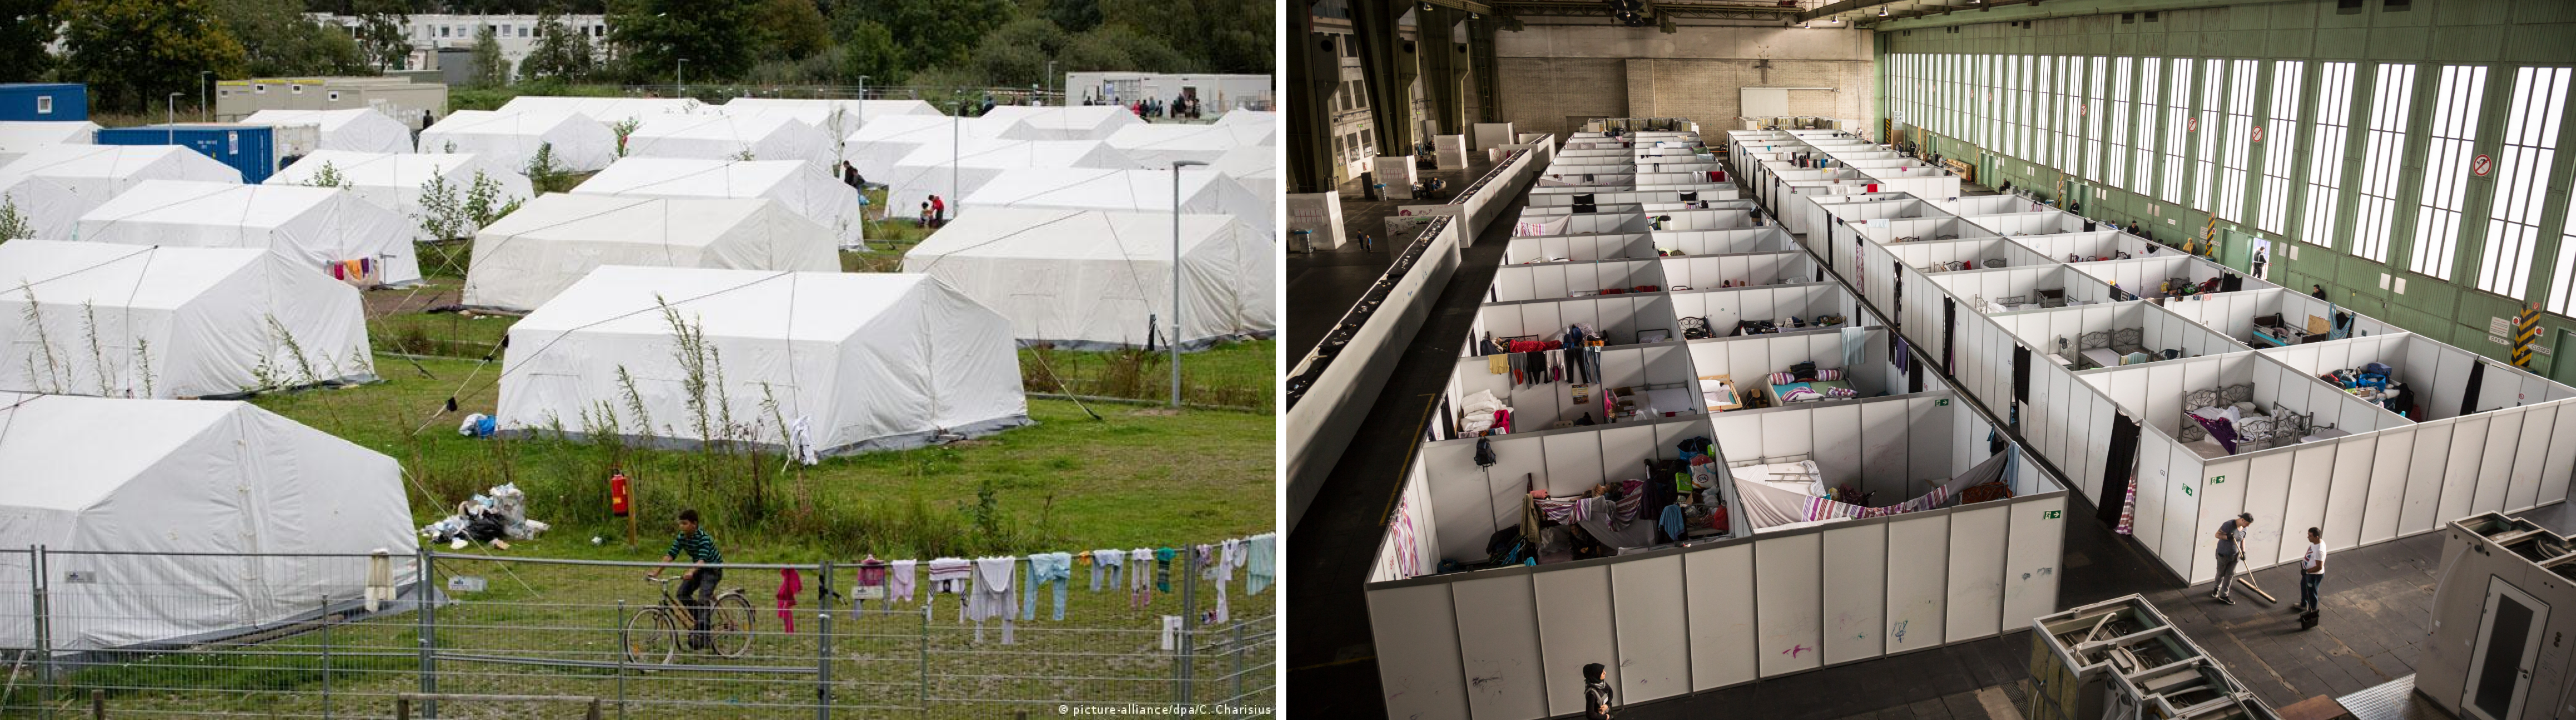
\includegraphics[width=1\textwidth]{chapters/consensus/findingplaces/figures/fp4.png}
            \end{center}
            \caption{
                Refugees in Germany, 2015. The influx of refugees and asylum-seekers during `15-`16 brought the German Government and local municipalities to seek quick solutions: Under-used facilitates, such as Berlin's Tempelhof Airport, were transformed into refugee camps; In Hamburg, tent-cities were constructed and empty properties were re-used in an effort to accommodate thousands of refugees. In most cases, these solutions could only offer short-term remedy, but were not suitable as long-term accommodations. Photo: C. Charisus, DW.com
            }
            \label{fig:fp_refugees_housing}
        \end{figure}


        In Hamburg, accommodation facilities concentrated in certain neighborhoods, while others received little to no refugees at all. Civil protest against refugee accommodation projects began to arise. Only few cases of physical hostility towards foreigners were reported, but nevertheless highlighted the civics' demand to be heard \cite{Antiraci26:online}. The heated and emotional debate motivated Hamburg's First Mayor to initiate a citizen dialogue and openly discuss where-and-how to accommodate refugees now and in the future. The idea was to address the issue as a collective, in which citizens themselves could take responsibility and contribute their knowledge towards a common solution. This participation process was given the name ``FindingPlaces'' (FP) \cite{Hamburge78:online}.
    }

    \subsection{Political Mandate and Goals}
    {

        \begin{figure}[!htb]
            \begin{center}
                \includegraphics[width=1\textwidth]{chapters/consensus/findingplaces/figures/fp6.jpg}
            \end{center}
            \caption{
                Inaugurating FindingPlaces. On May 11\textsuperscript{th} 2016, Olaf Scholz, (First Mayor of Hamburg `11-`18, Chancellor of Germany since `21), inaugurated the project and invited the public to take active role in setting their city's future: \textit{``FindingPlaces brings together the knowledge of residents, authorities and geographers and makes it immediately usable. The participants in the workshops are in the position of informed city planners who have to deal with an extremely complex task. It's not just any theoretical task, but the task that our city has to solve together: Which areas can we use to house refugees? FindingPlaces answers: This is your city! Here is your chance to examine whether what makes sense in theory, is also suitable in practice.''} (Excerpts from Olaf Scholz's speech, May 11\textsuperscript{th} `16, HCU) Also in this photo (from left to right): Katharina Fegebank, Second Mayor of Hamburg; Prof. Dr. Gesa Ziemer HafenCity Universität, Director CSL; Olaf Scholz, 1\textsuperscript{th} Mayor of Hamburg; Walter Pelka, frmr. HCU President; and Kent Larson, Dir. MIT City Science.
            }
            \label{fig:fp_olaf_scholz}
        \end{figure}


        In June 2015, The City of Hamburg and the MIT Media Lab signed a long-term research collaboration agreement that promoted the establishment of the City Science Lab (CSL) at HafenCity University Hamburg (HCU) \cite{HafenCit25:online}. In February 2016, CSL was assigned by then First Mayor Mayor Scholz\footnote{As of Dec. `21, Olaf Scholz is new German Chancellor, succeeding Angela Merkel} to develop a participatory process that would enable citizens to engage in finding accommodations for a predicted influx of nearly 80,000 refugees. The goal was to incorporate the citizens' personal experience and local knowledge into the political and administrative evaluation of potential locations, while creating a public discourse, innovation, and learning around the challenges of immigration. The results and proposals emerging from the participation process were to become recommendations for decision-makers and planning authorities. FP was developed in coordination with the Senate Office, the Central Refugees Coordination Staff (ZKF)\footnote{\url{https://www.hamburg.de/sfa-about-us/}}, district administration representatives, and the Hamburg Urban Development and Revitalization Agency (STEG)\footnote{\url{https://www.steg-hamburg.de/}}, who specialized in citizen participation processes. The mayor's office permitted three months for conception and development of FP. Figure \ref{fig:fp_olaf_scholz} shows the inauguration event of FindingPlaces by the First Mayor of Hamburg.
    }

    \subsection{Concept and Method}
    {
        Traditionally, decision-making for the allocation of refugees accommodations was mostly done by small groups of experts based on their technical, legal, and contextual knowledge \cite{sprandel2018housing}. FP required multidisciplinary expertise and methods to tackle the question of citizens' involvement in refugees' accommodations. To enable citizens' input, CityScope was proposed as a decision-making and knowledge-support tool, that can leverage the publics' insights in concert with evidence-based urban data, analytics, and predictions. A series of public participation workshops was planned to be centered around interactive CityScope stations, displaying data to citizen groups as they worked out decisions. The main conceptual components of FP included (i) A workflow design for the overall workshop series; (ii) A procedure for participatory workshops; (iii) The technical adaptation of CityScope interactive tools; and (iv) Extensive pre-processing of urban data.
    }

    \subsection{System Design}
    {
        The FP use-case presented a set of unfamiliar socio-technical challenges. Adaption of the CityScope to FP required major refactoring of the system, such as the introduction of networked communication between platforms, integration of a real-time Geographic Information System (GIS) service, as well as streamlined data , stability, and error mitigation. Workshops were designed to focus on one interactive CityScope table at a time, showing a user-selected part of the city on a scale of $1:750m$. Geographic data on Hamburg's parcels were augmented by several data layers, such as ownership models, land-use, environmental conditions, or hazards, to highlight places' suitability for refugee accommodation.

        \subsubsection{Data}
        {
            To evaluate the availability of a parcel for refugee accommodation, detailed information about Hamburg's land uses and land distribution was required. Different spatial data sources were aggregated into the GIS database, such as parcels ownership model, current uses of parcels, and existing development constraints, such as nature reserves or land contamination. These geospatial layers were sorted into three ranked classes:

            \begin{itemize}
                \item{
                            \textbf{High indication of unsuitability}: Places significantly affected by highly restrictive criteria, such as nature conservation, cemeteries, places under significant noise emission, etc.
                      }
                \item{
                            \textbf{Medium indication of unsuitability}: Places insignificantly affected of aforementioned highly restrictive criteria but still affected by less restrictive criteria like parks, designated recreational areas, proximity to high-voltage power lines or similar.
                      }
                \item{
                            \textbf{Low or no indication of unsuitability}: Places not affected by highly restrictive criteria with less restrictive criteria affecting less than 50\% of the area.
                      }

            \end{itemize}
            These classes were set to provide a baseline for the selection of places discussed during a workshop. For viewing purposes, additional geospatial data hosted by external providers was integrated as cascaded WMS in GeoServer (e.g., aerial imagery of Hamburg) or client-side tile layers in OpenLayers (e.g., OpenStreetMap).
        }

        \subsection{User Interaction}
        {
            Using CityScope, participants could place a specific LEGO tile onto the TUI, and query attributes of the underlying geospatial data. A selection of tiles assigned to different pre-defined housing attributes, could be placed to add a proposed numbers of accommodations to a certain parcel. The results of these interactions were visualized on auxiliary displays, using maps of different scale and granularity, diagrams and statistics. For example, if a user placed a tile representing an accommodation capacity of 25 families, its location and density would be displayed on the table itself, on a map projected onto another table featuring the entire district, as well as on a regional map of Hamburg.
            \newline
            In addition, different diagrams and statistics, representing the total accommodation capacity for a specific district, as well as for the entire city of Hamburg, would be displayed on nearby monitors.
            Aside from the interactive TUI, a second table was used to depict a dynamic overview map of the specific district under consideration during workshop. Both tables were illuminated by a pair of projectors, each covering a half; Auxiliary displays were handled by large TV screens with a wall-mounted canvas showing a global overview of FP statistics and information.
        }

        \subsubsection{Computation}
        {
            Each CityScope table was equipped with a workstation, driving the nearby displays and projectors. The workstation at the district table was used to perform backend operations, such as image recognition and GIS server communication; The workstation at the interactive table was used to control the map displays; The GIS server was hosted on a virtual machine on the HCU's servers. Similar to other CityScopes, FP computation module included three main components: (i) Image processing of live video data for the interpretation of user-interactions; (ii) Translation and processing of these inputs into a geospatial context (GIS); and (iii) Analysis and visualization of the effects of recorded interaction. The following Subsections describe the main components of FP computation.
        }

        \subsubsection{TUI and Scanning}
        {

            \begin{figure}[!htb]
                \begin{center}
                    \includegraphics[width=1\textwidth]{chapters/consensus/findingplaces/figures/fp7.png}
                \end{center}
                \caption{FindingPlaces TUI Scanning Module: Processing of a video frame to GIS query. FindingPlaces utilized 4 webcams to capture the overall table state; The captured image would then be processed to allocate colored tiles, and project them onto a geographic coordination system. Finally, tiles found to match a designated site would add or subtract housing capacity in that area, thus affecting the overall housing count.}
                \label{fig:predictions_scan}
            \end{figure}

            the TUI utilized few regularly shaped, color-coded LEGO tiles on a plexiglass grid \eqref{subsec:csarch-cityscopy}. All other grid cells were filled with low, neutrally white objects that provided a canvas for the map display via the overhead projectors. In order to scan the entire surface of the CityScope TUI simultaneously, an array of four web-cameras was used, each one covering a square quarter of the table. Image recognition was handled by two single-board mini-computers which streamed the video from the webcams to a workstation computer. The single-board scanning units ran \texttt{ffserver} and \texttt{ffmpeg} to stream their video feeds to the network. Video processing and interpretation were implemented using the computer vision library \texttt{OpenCV} and \texttt{numpy} \cite{opencv_library}.
            \newline
            Shapes visible in the webcam video feed were then analyzed and compared against a lookup table of known brick color-codes. The data attributes and coordinates of successfully detected bricks were then transmitted and translated it into the GIS context. The GIS server was then queried for the attributes of the bricks, computed the new state, and displayed the results on the different output devices. Figure \eqref{fig:predictions_scan} illustrates the scanning process and GIS geo-projection.
        }

        \subsubsection{Software}
        {
            The specialized software for the FP project included microservice-like architecture. The majority of communication between processes was handled using a publish-subscribe pattern built on a Crossbar router with \texttt{Autobahn.JS} and \texttt{Autobahn-Python} clients using WebSockets for asynchronous processing. The main GIS server was a GeoServer instance, with its data managed in a \texttt{PostgreSQL} and \texttt{PostGIS} database. Map display on the tables was done via OpenLayers clients in web-browser windows. Data transfer and spatial queries between the GIS server and the clients were performed via GeoServer's \texttt{WFS API} using the Python bindings of OGR/GDAL, while specific non-spatial queries were run directly against the database. The backend was developed in Python, and the frontend with standard web technologies \texttt{JavaScript, HTML, and CSS}.
        }

    }

    \subsection{Participation Campaign}
    {
        Between May and July 2016, a total of 34, two-hour workshops were held at HafenCity University campus, totalling nearly 400 participants. Each workshop focused on one of the city's seven districts, and participants were specifically invited based on their prior knowledge of these areas. The workshops were advertised via various media channels and $\sim$40,000 brochures distributed all over the city, having an estimated reach of $\sim$5 million citizens. Participants were asked to register online and $\sim$20 people per session were eventually invited; On average, 11 people participated per workshop. Participants could only attend one workshop per district, while response and registration numbers varied based on each district. The diverse range of participants was characterized by a strong heterogeneity concerning age, profession, political views, social values, and personal motivation to participate.


        \begin{figure}[!htb]
            \begin{center}
                \includegraphics[width=1\textwidth]{chapters/consensus/findingplaces/figures/fp8.png}
            \end{center}
            \caption{FindingPlaces - CityScope Setup. Amongst other contributions, FindingPlaces was the first interconnected CityScope system that linked user-interactions and data from multiple instances, and utilized it in all other places. This created a sense of continuation between the different Stations, as participants could observe their previous actions reflected in other stations.}
            \label{fig:predictions_setup_overall}
        \end{figure}

        \subsubsection{Venue and Moderation}
        {
            The workshops took place from Monday to Saturday at a gallery space of 150$m^2$ on HCU entrance floor. This site was deliberately chosen for being considered a neutral location in the city for the often emotionally charged discussions on refugee accommodations. A team of six to eight people was in charge of the organization and conduct of each workshop: one moderator leading the discussion, one assistant documenting the exchange, one researcher accompanying the workshops for scientific purposes, one technical staff operating the equipment, and one or two representatives each from the Central Refugees Coordination Staff and district administration. The moderators were leading the workshops, while other team members provided on-demand details concerning the CityScope system, specific sites, or information regarding refugees' accommodation in general. In later review, it was mentioned that the open discussion contributed to the participants' grasp of the complex subject matter. Figures \eqref{fig:fp_session} and \eqref{fig:predictions_setup_overall} show a typical workshop setup at the HCU venue.
        }
    }

    \subsection{Workshop Procedure}
    {
        Similar to the BRT project \eqref{sec:brt}, the venue was divided into three stations, displaying different scales of the city: Hamburg City region, district, and neighborhood.

        \subsubsection{(i) Hamburg City}
        {
            At first, an intro video was shown to inform participants about the workshop procedure, the current condition of refugees, and the challenge of providing appropriate accommodation. The general task was presented: `Which city-owned parcels would be suitable locations for refugee accommodation?' The goal was to find sites that in total could accommodate nearly 20,000 refugees and thus meet the predicted demand until the end of 2016\footnote{Total predicted newcomers varied significantly during 2015-2016. Geopolitical shifts, such as border closures and stricter migration control in eastern states changed Hamburg's predictions over time \cite{katz2016cities}. Nevertheless, the goal of FP was to build a pool of sites not only for current newcomers, but also for potential future ones.}. The locations of all existing and planned refugee accommodations were shown on a map, as well as the current statistics on the refugee distribution to the different districts. In addition, the targeted number of accommodation places was displayed, counting down in real-time in response to new locations proposed by the participants during the workshops.
        }

        \begin{figure}[!htb]
            \begin{center}
                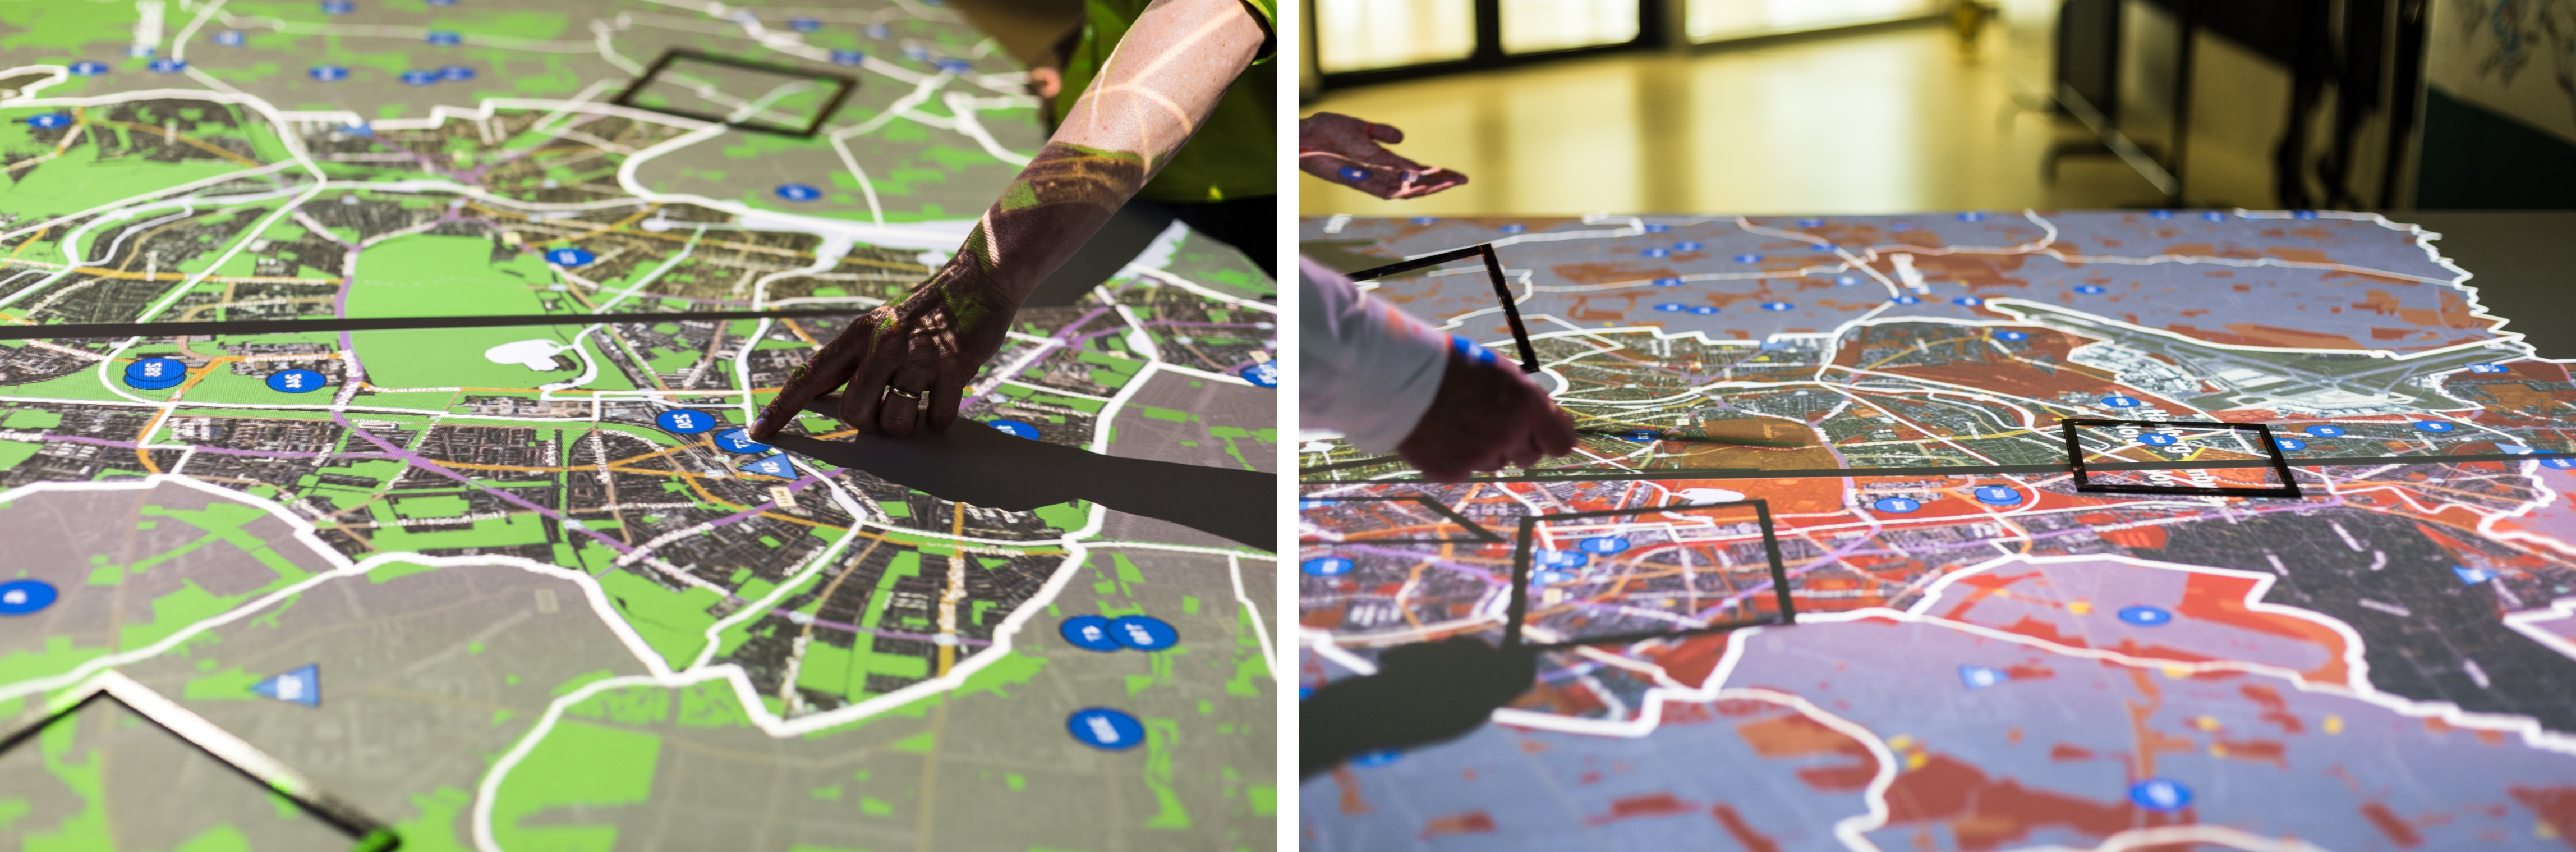
\includegraphics[width=1\textwidth]{chapters/consensus/findingplaces/figures/fp2.png}
            \end{center}
            \caption{
                Regional and District Scales. This CityScope instance showed the locations of existing and planned refugee accommodations, including their actual occupation rates were indicated. Available places were colored: $Red$ for places with a high indication of unsuitability, $orange$ for a medium indication, and $yellow$ for likely suitable places. Further information on the number of inhabitants and refugees currently accommodated in the district was presented on a screen.
            }
            \label{fig:fp_city_scale}
        \end{figure}


        \subsubsection{(ii) District}
        {
            After the introduction, the first CityScope table was introduced. Here, a satellite image projected onto the table showed the city district at stake. Street and neighborhood names, as well as distinctive points of interest, were displayed to provide orientation. As with the city scale, the locations of existing and planned refugee accommodations, including their actual occupation rates were indicated. Available places were colored according to their previously determined suitability classes: $Red$ for places with a high indication of unsuitability, $orange$ for a medium indication, and $yellow$ for likely suitable places. Further information on the number of inhabitants and refugees currently accommodated in the district was presented on a screen. Taking into account that not all spaces could possibly be discussed during the two-hour workshop, the participants were asked to select focus-areas for the next station. Selection criteria could be specific knowledge of a place, the need for equal distribution of refugees within the city, or the color-index of the spaces. Figure \eqref{fig:fp_city_scale} shows the locations of existing and planned refugee accommodations, as well as areas which can be considered for allocation of new housing.
        }


        \begin{figure}[!htb]
            \begin{center}
                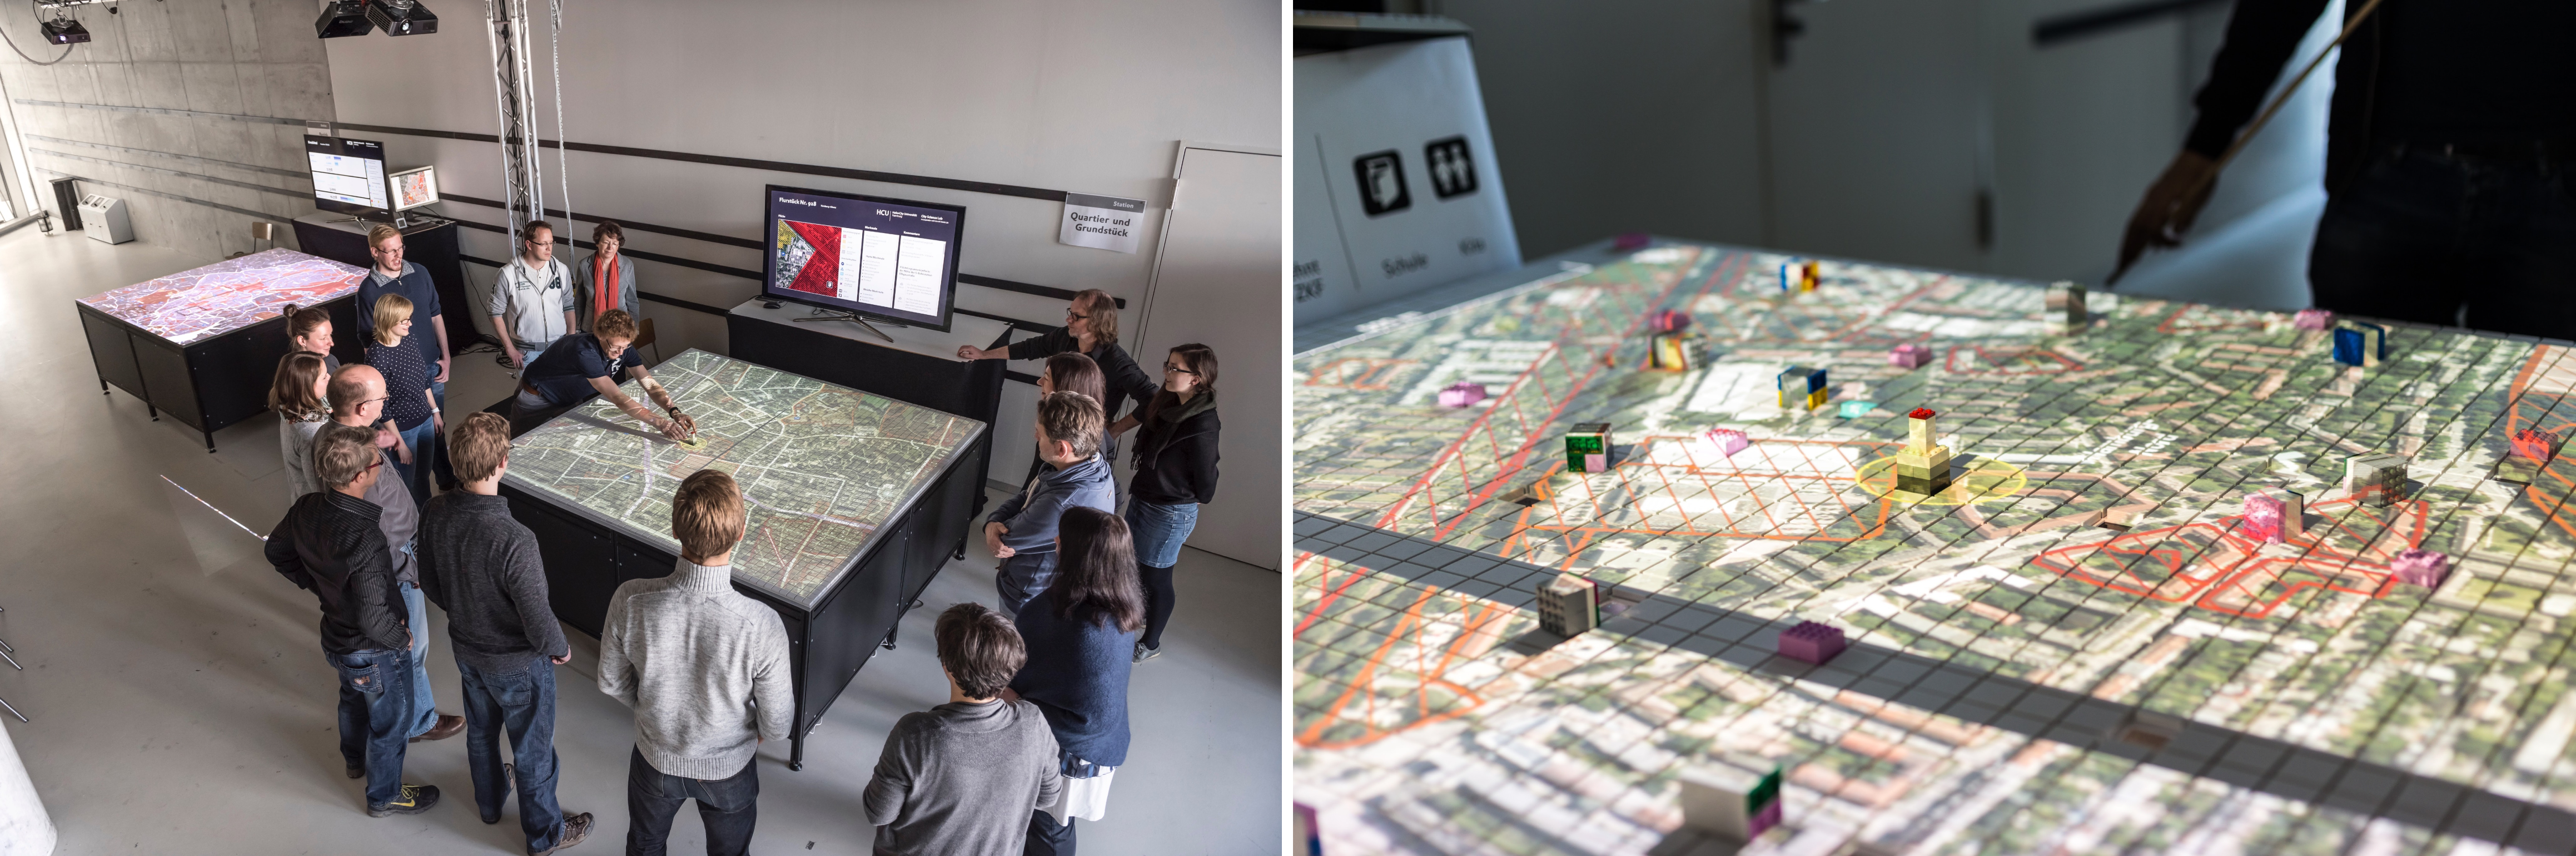
\includegraphics[width=1\textwidth]{chapters/consensus/findingplaces/figures/fp5.png}
            \end{center}
            \caption{
                Neighborhood Scale. After observing the regional scale, a chosen focus area was projected on an interactive CityScope, in which participants were able to identify details such as buildings, parks or playgrounds. By placing a marker piece onto a parcel, the potential accommodation capacity for the site was indicated. Additionally, area in $m^2$, planning regulations, and restrictions such as nature conservation, biotope, or high-voltage lines, were presented. When participants reached a consensus and identify a location suitable for refugee accommodation, another marker piece was placed on the TUI, indicating the number of accommodation places (40 - 1,500); the screens and the CityScope at the Hamburg and district-stations were also displaying the location of the suggested parcel. Photo: W. Schieswohl, author.
            }
            \label{fig:fp_neighborhood_scale}
        \end{figure}


        \subsubsection{(iii) Neighborhood}
        {
            The chosen focus areas were projected onto the second interactive CityScope, with the suitability classes shown in colored hatching. At this scale, participants were able to identify details like buildings, parks or playgrounds. In addition to refugee accommodations, social infrastructure like kindergartens or schools, as well as bus or train stops was shown. By placing a marker piece onto a parcel, detail information on the property was displayed on a screen, including area in $m^2$, planning regulations, designation of the area, as well as restrictions such as nature conservation, biotope, or high-voltage lines. Additionally, the potential accommodation capacity for the site was computed and indicated. Participants' verbal discussion of the pros and cons for each parcel were logged and displayed on the screen.
            \newline
            When participants reached a consensus and identify a location suitable for refugee accommodation, this parcel could be suggested and forwarded to the city officials. To do so, another marker piece was placed on the TUI, indicating the number of accommodation places (between 40 to 1,500). At that point, the screens and the CityScope at the Hamburg and district-stations were also displaying the location of the suggested parcel. Finally, the proposed number of refugees was included in the system's statistics. Figure \eqref{fig:fp_neighborhood_scale} shows the interaction with the Neighborhood Scale TUI.
        }
    }

    \subsection{Results}
    {

        \begin{figure}[!htb]
            \begin{center}
                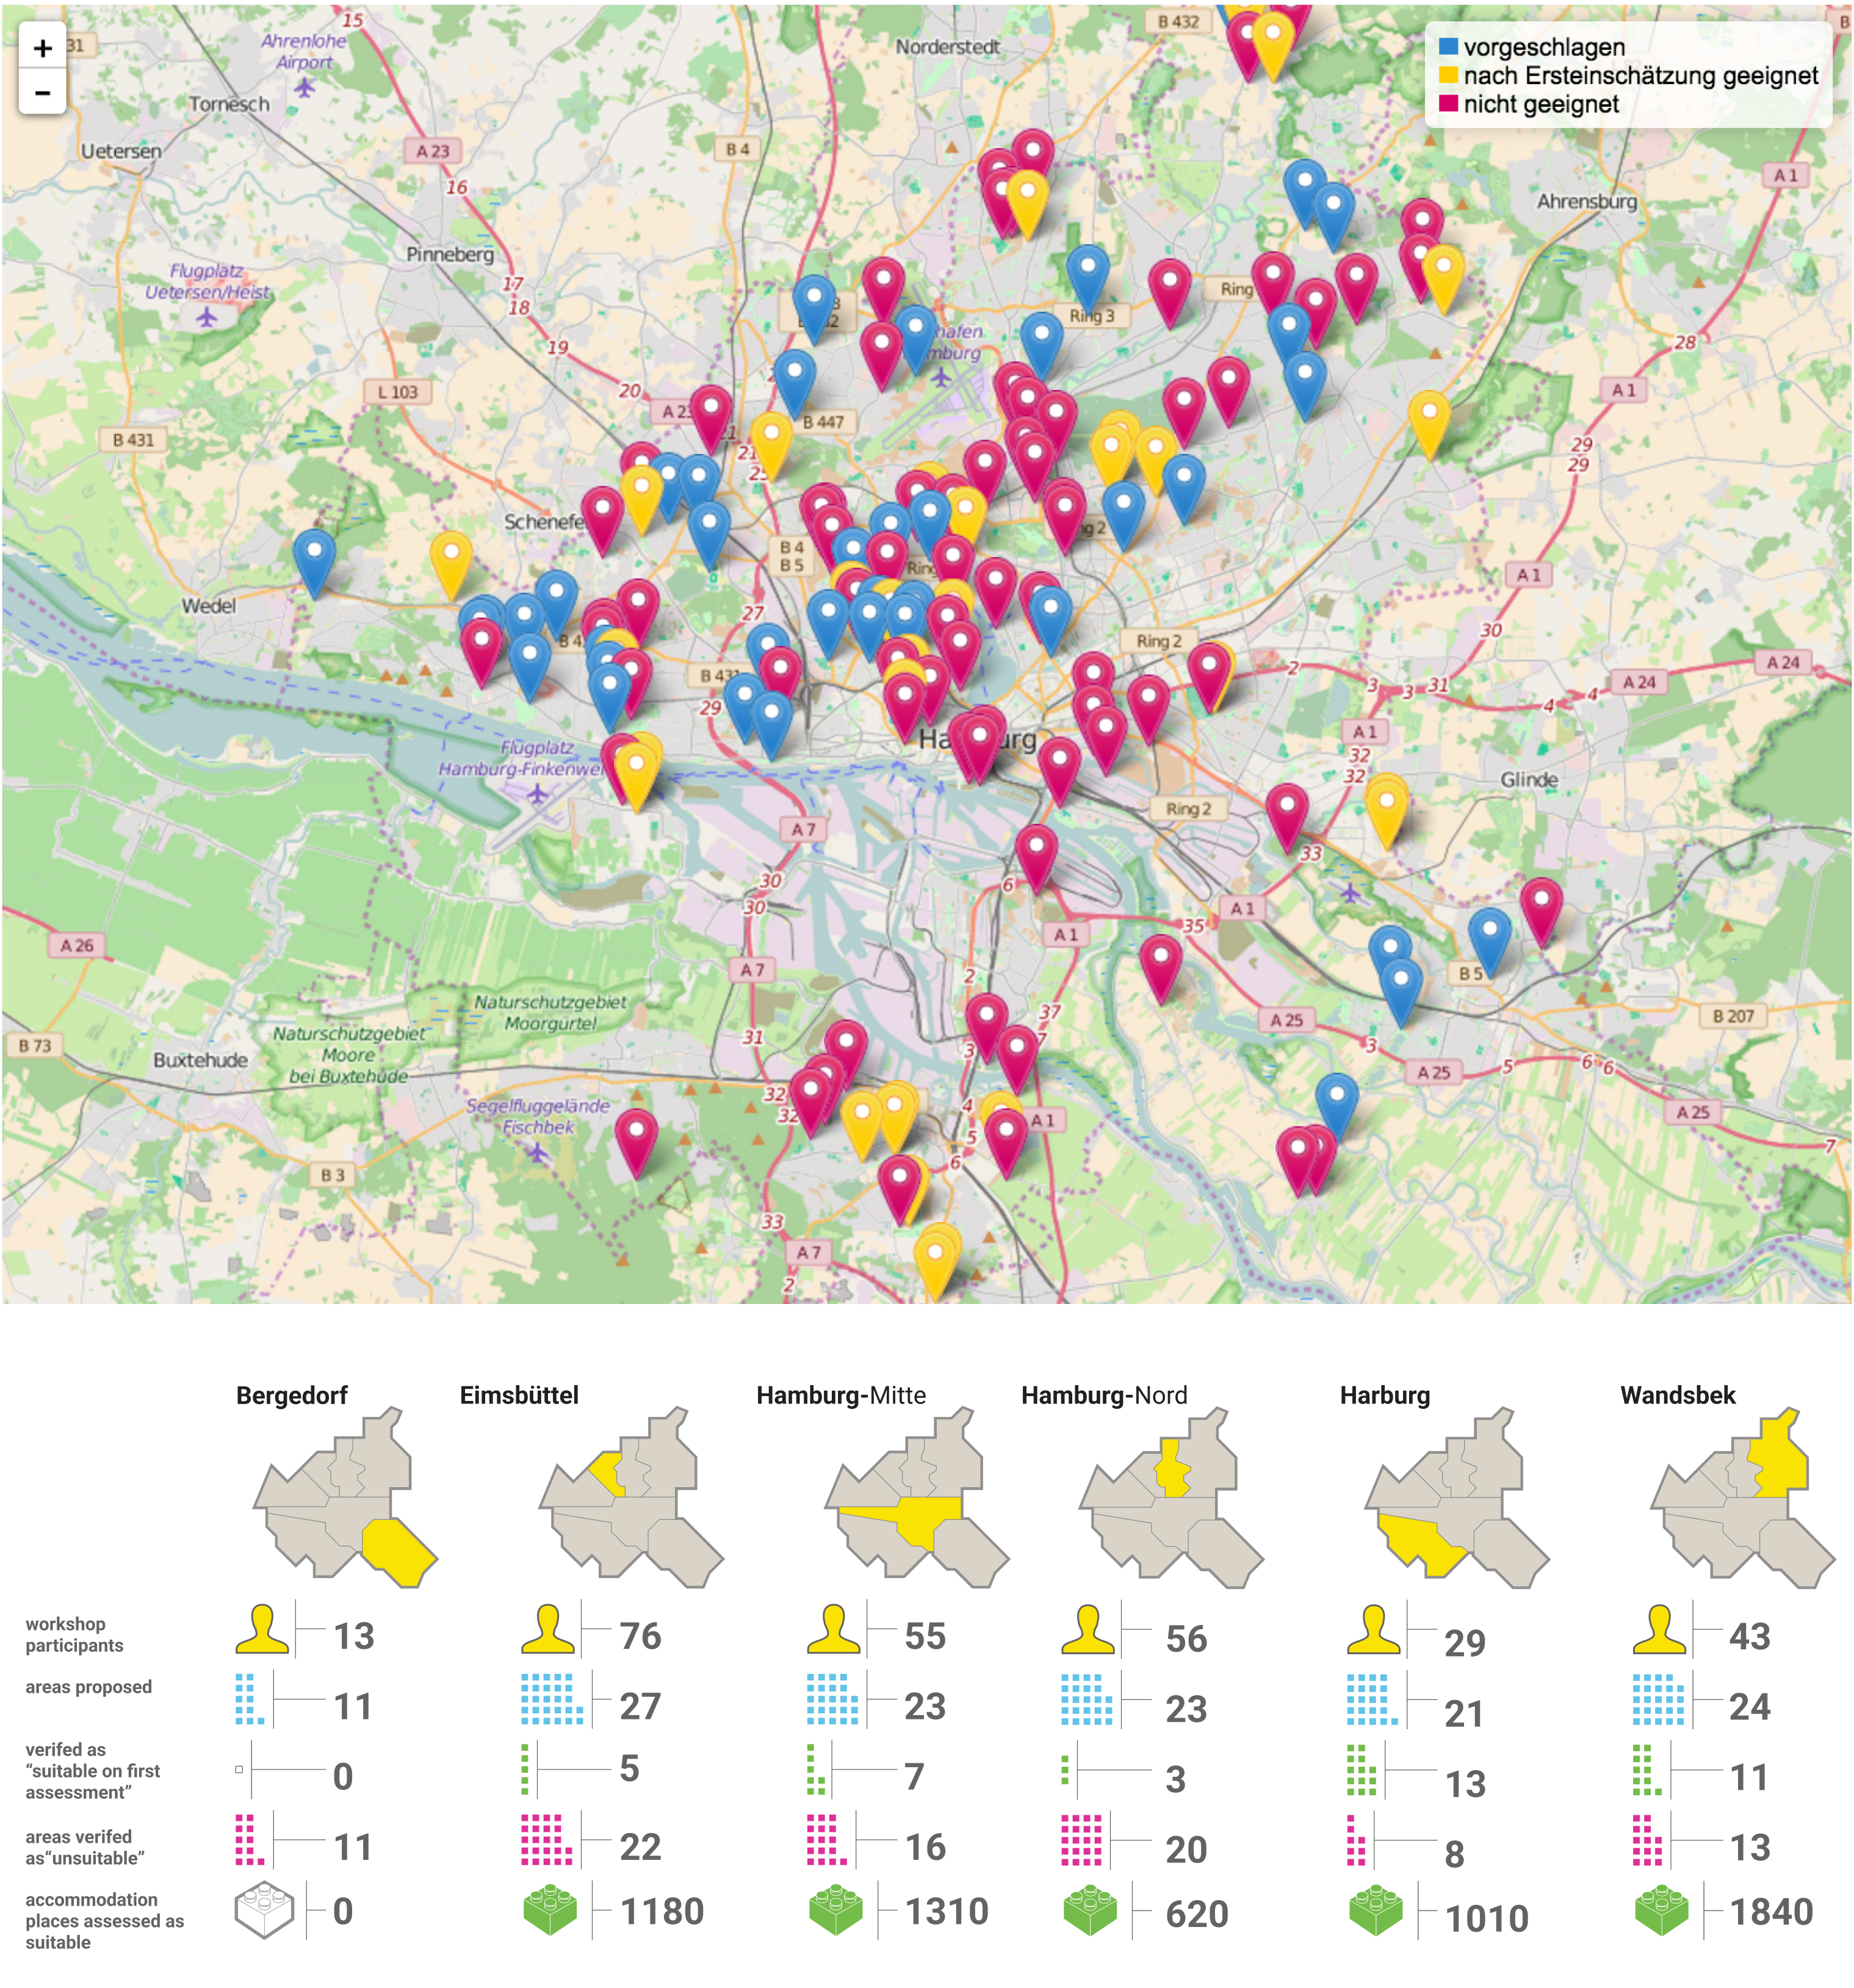
\includegraphics[width=1\textwidth]{chapters/consensus/findingplaces/figures/fp1.png}
            \end{center}
            \caption{FindingPlaces results. (top) The map marks the total places found by community members. The colors present `suggested to approval' (blue), `to be further investigated' (yellow), or `not suitable' (red). Importantly, the map demonstrates the rather equal distribution of places found by the general public, which solidifies the sense of general acceptance of asylum seekers amongst diverse neighborhoods. (bottom) Breakdown of results per each administrative district. Photo: FindingPlaces, HCU}
            \label{fig:fp_results}
        \end{figure}

        At the end of each workshop, a list of the agreed upon parcels was delivered directly to the Central Refugees Coordination Staff, along with all information regarding the planning restrictions and transcripts of the discussion. These materials were also uploaded to the official FP website for public access. The Central Refugees Coordination Staff would then initiate a screening process, in which each suggested parcel went through a rigorous feasibility test. The results of this process were published online within two weeks; Parcels which were deemed suitable were then further studied by the city's planning authorities.

        \subsubsection{Allocated Sites}
        {
            In total, 161 locations were suggested by the participants and evaluated by the authorities. With these, accommodation solutions for nearly 24,000 refugees were proposed, exceeding the initial targeted goal of 20,000. More than half of the parcels were designated parks, green areas in inner-city locations, landscape, or agricultural spaces in rural areas, that are mostly subject to nature or landscape conservation. Another 15\% of the suggested parcels were used as sports fields or playgrounds. Others were parking lots, commercial and industrial areas, parcels designated for future housing projects or port area parcels. Almost three quarters of the suggested locations were rated as not suitable in the initial assessment, leaving 44 rated as feasible. A further 24 were excluded after a detailed examination. Ultimately, 6 received recommendations for implementation and 10 were taken into consideration for future planning. In these lasting 6 locations, approximately 750 refugees could be accommodated, 4\% of the initial target. Figure \eqref{fig:fp_results} shows the places found across the regional area of Hamburg, and a breakdown of the results per district.
            \newline
            Several reasons led to rejections of allocated sites: More than a third of the parcels were not available due to the existence of other land-uses, such as commercial activities or sport and leisure purposes. Another third of the parcels could not be used due to direct conflicts of land-use, mostly parks and playgrounds. Other reasons for rejection were of technical or structural nature, such as hazardous environment, contamination, topographic constraints, protection of historical monuments, or a lack of nearby transit and social infrastructure.
        }

        \subsubsection{Interaction Process}
        {
            The FP workshop methodology motivated a high degree of involvement and direct discussion between experts and non-experts. Despite the emotional charge and heated public debate concerning refugee accommodations, the discussions and atmosphere in the workshops were mostly constructive. Occasionally, participants expressed their dissatisfaction with the refugee policy pursued by the Hamburg senate. Some were arguing that FP might have been a dishonest participation process, only utilized to restore peace in the city.
            \newline
            However, it could be observed that the disapproving comments were mostly based on vague or incorrect information, and were hence quickly diminishing with the provision of more precise information. This highlighted that the dialogue between the participants could be quickly rationalized by shifting from a theoretical discussion to a more tangible level, through the usage of clear information and facts. For example, participants could not simply reject a proposed parcel without providing arguments that were clear to other participants. During the workshops, many ideas of an ideal solution for refugees accommodation had to pass a `reality check', pushing some to be revised as they were incompatible with the applicable planning regulations and site restrictions.
        }
    }

    \begin{figure}[!htb]
        \begin{center}
            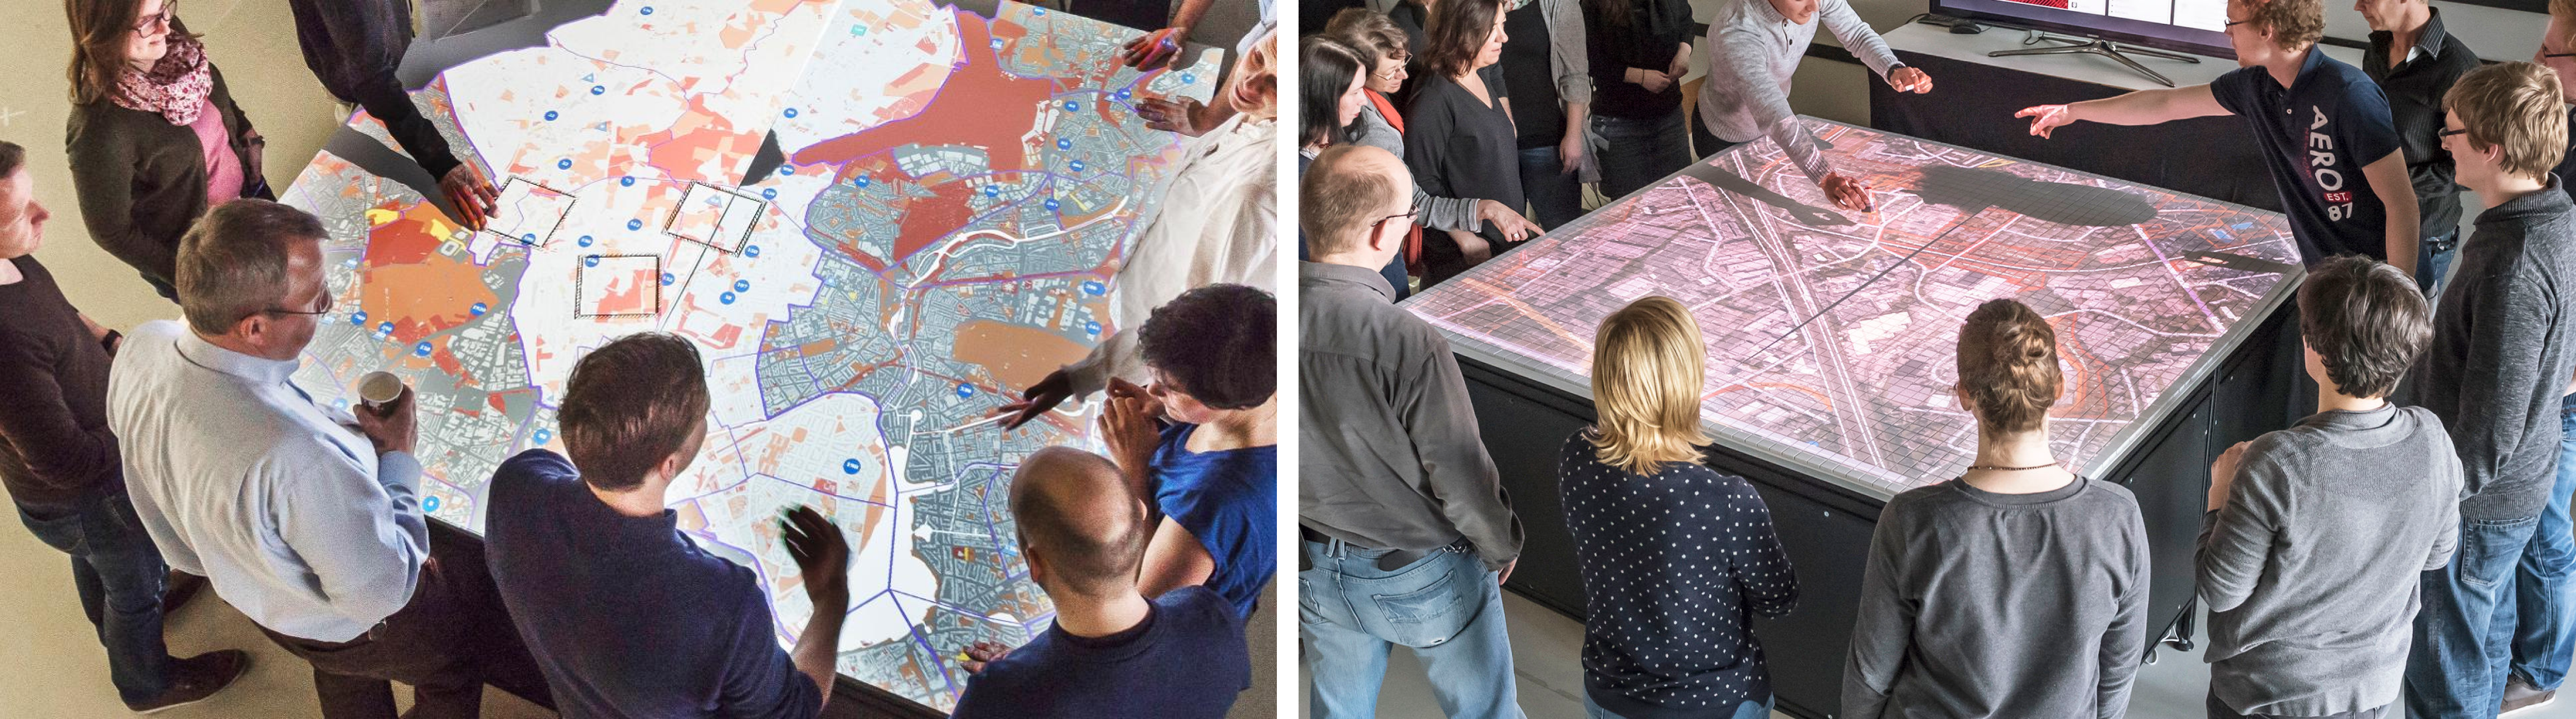
\includegraphics[width=1\textwidth]{chapters/consensus/findingplaces/figures/fp3.png}
        \end{center}
        \caption{
            Participation and engagement. As with the Boston BRT project \eqref{sec:brt}, the FindingPlaces CityScope's were designed as a literal common-ground, in which technology is only set to encourage a vibrant public discourse. The tables were sized to accommodate a large number of participants, and the groups were able to interact freely with the system. Extra effort was made to ensure disabled and elderly participants were not disadvantaged; Nevertheless, the system presented a degree of visual complexity not always suitable for the general public. Photo: W. Schieswohl, City of Hamburg, HCU.
        }
        \label{fig:fp_engagement}
    \end{figure}

    \subsection{Discussion}
    {
        By both stakeholders and participants, FP was evaluated as a highly positive experience, and CityScope was recognized to greatly support public participation and real-time decision-making. It was noted that citizens felt as partners in an `eye-level' dialogue with policy-makers and city administration, being able to supply planning authorities with relevant information based on their local knowledge. The project built up acceptance towards refugee accommodation in Hamburg, and triggered high-quality feedback in comparison to other public discussions at the time. Making administrative procedures and decisions transparent effectively contributed to the `political literacy' of the general citizenship.

        \subsection{Limitations}
        {
            A key challenge of FP was the tight schedule in which the project needed to be implemented and communicated to the general public. Logistical limitations reduced the overall exposure of the CityScope tool: Due to the size of the platform, workshops were bound to be held at HCU campus instead of closer to participants' locations. This naturally reduced the number of potential participants, thus contributing to a selection bias which favored more mobile and capable members of the community \cite{Innes2016}.
            \newline
            Another constrain was the form of representation of urban data: Despite thorough pre-processing, non-expert participants had trouble understanding the professional planning content, which was not distilled enough for the general public. As participants were not used to working with maps or satellite images, orienting the projected images and assessing them adequately was challenging. Figure \eqref{fig:fp_engagement} shows the engagement of participants in the workshop, and the potential complexity of the FP data visualization.
            \newline
            Lastly, sites that were eventually deemed unsuitable, were not immediately removed from the system, but rather were evaluated by the planning authorities at a later stage. This meant that the system was not able to provide a clear picture of the feasibility of proposed sites in real-time, thus reducing the number of sites that were eventually approved. In future versions of such system, pre-approval or rejection of simple sites (i.e., sites with clear feasibility indication) should be automated.
        }
    }

    \subsection{Conclusion}
    {
        Refugees and global immigration waves remain a major challenge of high urgency all across the world. Global socio-political developments may yield new migrant waves, and the accommodation of refugees in `arrival cities' remains acute. The usage of CityScope in this context, demonstrated how socio-technical platforms can effectively support consensus-building and trust amongst the public. It highlighted the importance of gaining `street-knowledge' and crowd-sourced perspective, while validating it with facts, data, and information. CityScope served this project in two ways: It assisted with fast and accurate decision-making, by methodically allocating and evaluating housing solutions. But more broadly, CityScope FP was acting as an amplifier which echoed the public's voice, helping them to collectively discuss, design, and shape their own urban future.
    }
}
    %%%%%%%%%%%%%%%%%%%%%%%%%%%%%%%%%%%%%%%%%%%%%%%%%%
    
    \section{Discussion: Consensus Building}\label{sec:cons-decentralizing}
    {
        This chapter discussed CityScope's role in consensus-driven processes for urban decision-making. Previous chapters have shown how CityScope is designed for an evidence-based, iterative, and collaborative planning process; Yet these advantages cannot promise a truly participatory process. In fact, many of the technological features presented in previous chapters might improve the quality of traditional planning, but thus negate a consensus-driven process. For example, an iterative design platform could be used by a planning authority to improve the design outcome of a neighborhood, but it would not be utilized in a public-facing manner; location data might support regulatory amendments, but these data and models might not be accessible to the rest of the community for critical evaluation.
        \newline
        The work presented in this Chapter emphasized the need to coverage the advantages of urban technologies with a public-facing social discourse. As evident from work reviewed in this and prior Chapters, collaborative UHCI systems can only benefit their communities if they themselves are open for review, evaluation, and even criticism. This type of `technological consensus' has the potential to elevate legally-binding public participation towards true partnership and citizen control \cite{arnstein1969ladder, Innes2016}.
    }
}

